\section*{ГЛАВА 4\\ ОСОБЕННОСТИ РЕАЛИЗАЦИИ ОБРАЗОВАТЕЛЬНОЙ ПЛАТФОРМЫ}
\setcounter{section}{4}\setcounter{subsection}{0}
\addcontentsline{toc}{section}{ГЛАВА 4}
\addcontentsline{toc}{section}{ОСОБЕННОСТИ РЕАЛИЗАЦИИ ОБРАЗОВАТЕЛЬНОЙ ПЛАТФОРМЫ}


В данном разделе описаны детали реализации приложения, а также приведены результаты его тестирования.
В ходе работы над проектом необходимо было реализовать модульные компоненты, которые позволили
бы в дальнейшем минимизировать трудозатраты на доработки и расширение системы.

\subsection{Структура приложения}

После анализа возможных вариантов реализации приложения, была выбрана многоуровневая архитектура,
каждый уровень отвечает за свою логическую часть.

В стандарте IEEE 1471 дается следующее определение: «Архитектура – это базовая организация
системы, которая описывает связи между компонентами этой системы (и внешней средой),
а также определяет принципы её проектирования и развития». Однако многие другие определения
архитектуры признают не только структурные элементы, но и их композиции, а также интерфейсы
и другие соединительные звенья.

Многоуровневая архитектура – является одной из самых известных архитектур, в которой
каждый слой выполняет определенную функцию. В зависимости от ваших нужд вы можете
реализовать любое количество уровней, но слишком большое их количество приведет к
чрезмерному усложнению системы. Часто выделяют три основных уровня: уровень представления,
уровень логики и уровень данных.

Слою не обязательно знать, что делают его соседи. Здесь проявляется такое свойство как
разделение ответственности. Если все три слоя являются закрытыми, то запрос пользователя
к верхнему уровню инициирует цепочку обращений с верхнего уровня до самого нижнего.
В этом случае уровень представления отвечает за пользовательский интерфейс и отображение
данных для пользователя и ничего не знает о существовании физического хранилища данных.
Ничего о существовании базы данных не знает и уровень логики – его «беспокоят» только
правила бизнес-логики. Доступ к базе данных имеет лишь через уровень управления данными.

Достоинствами применения такой архитектуры являются простота разработки
(в основном из-за того, что этот вид архитектуры всем знаком) и простота тестирования.
Среди недостатков можно выделить возможные сложности с производительностью и масштабированием –
проблема в необходимости прохождения запросов и данных по всем уровням
(в том случае, если все слои являются закрытыми).

Presentation layer (уровень представления): это тот уровень, с которым непосредственно
взаимодействует пользователь. Он включает компоненты пользовательского интерфейса, механизм
получения ввода от пользователя. На данном уровне расположены представления и все те компоненты,
который составляют пользовательский интерфейс (стили, статичные страницы html, javascript),
контроллеры, объекты контекста запроса.

Business layer (уровень бизнес-логики): содержит набор компонентов, которые отвечают
за обработку полученных от уровня представлений данных, реализует всю необходимую
логику приложения, все вычисления, взаимодействует с базой данных и передает уровню
представления результат обработки.

Data Access layer (уровень доступа к данным): хранит модели, описывающие используемые сущности,
также здесь размещаются специфичные классы для работы с разными технологиями доступа к данным,
например, класс контекста данных Entity Framework, репозитории, через которые уровень
бизнес-логики взаимодействует с базой данных.

\subsection{Структура базы данных}

В качестве базы данных для разрабатываемого приложения была выбрана PostgreSQL.

В качестве примера на рисунке \ref{db} приведена часть базы данных отвечающая за хранение
видео.

\begin{figure}[H]
  \centering
  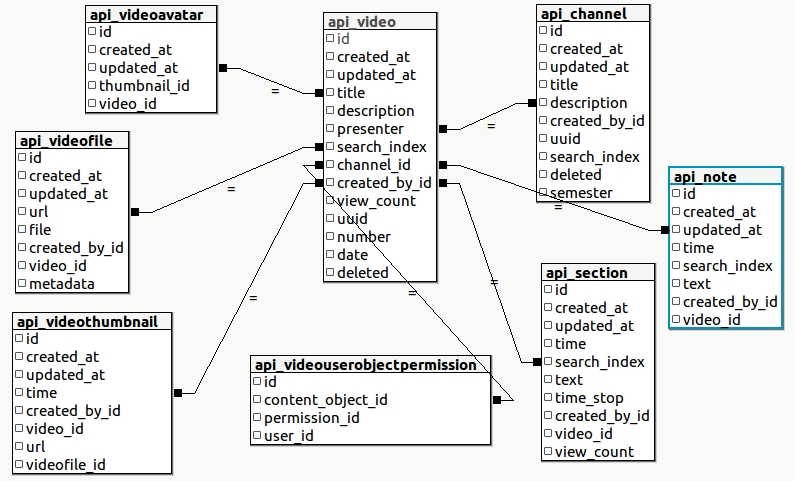
\includegraphics[width=1\textwidth]{images/db.jpg}
  \caption{Структура базы данных для хранения видео\label{db}}
\end{figure}


Данная структура позволяет хранить описание этих объектов такое как: тип объекта,
набор его полей, с указанием типа полей, а так же заданием особого поведения для
некоторых полей объекта.

Основные сущности были выделены в отдельные таблицы, структура базы данных включает
все необходимые элементы для эффективного хранения и представления данных приложения,
при необходимости она может быть легко расширена.

\subsection{Разграничение прав доступа}

Во многих проектах требуется реализация гибкого управление доступом на уровне записей (объектов), когда разные
пользователи имеют, или наоборот, не имеют доступ к отдельным объектам в рамках одной и той же модели. Для образовательной
платформы необходимо было разграничить доступ к загрузке, просмотру и аннотированию видеолекций.

Первоначально задумывалось реализация прав только на определение видимости объектов, разделяя их множество "по горизонтали".
Права управления объектами, попавшими в зону видимости, распределялись согласно традиционной системе прав в Django,
в соответствие с их моделями (типами) — "по вертикали". Такое разделение работало до определенного момента вполне приемлемо,
однако когда потребовалось распределять доступ "перекрестно", обнаружилось, что наша система слишком груба.
Действительно. Пусть мы распределяем доступ к объектам пользователей. Пользователь — админ своего канала, вполне может
отредактировать и даже удалить видео с этой канала. С другой стороны, хотелось бы, чтобы пользователи, которые являются
админами своих каналов, могли быть рядовыми пользователями других каналов. Однако, админ имеет одинаковый доступ к записям,
как только видит их, не важно, в какой группе.

Таким образом, стало ясно, что "по горизонтали" нужно управлять не только видимостью объектов, но и всем спектром операций,
производимых над ними. Таким образом в реализованной системе объектами стали выступают следующие сущности:
\begin{itemize}[wide,topsep=0pt]
  \itemsep0em
  \item аннотация (блок или секция)
  \item видеофайл
  \item канал
  \item пользователь
  \item группа пользователей
\end{itemize}
Для перечисленных объектов было реализовано управление со следующими доступами:
\begin{itemize}[wide,topsep=0pt]
  \itemsep0em
  \item просмотр
  \item редактирование
  \item аннотирование
  \item проигрывание
\end{itemize}

\subsubsection{Создание правил ограничения доступа}

Приложение реализует проверку прав на объект, а не на всю модель (object-level permissions) c помощью Django-Guardian.
Django-Guardian, требует создания нетипизированных отношений (то есть записей в БД) между пользователем и объектом,
с которым пользователь может взаимодействовать. Каждая пара пользователя и объекта требует такой отдельной записи о правах.
Количество этих записей в базе будет исчисляться, как произведение количества пользователей и объектов,
права доступа к которым регулируются в такой системе.
Начиная с Django 1.2 бэкенд аутентификации поддерживает проверку прав на объект, но это не реализовано в самом Django.
Django-Guardian успешно заполняет этот пробел. Пример описания прав доступа к видеообъекту
приведен в листинге ~\ref{lst:permissions}:

\begin{lstlisting}[caption={Пример описания прав доступа}, label=lst:permissions]
class ChannelVideoPermissionContext(dict):
  def __init__(self, user_permission_context):
    self._pc = user_permission_context
    super(ChannelVideoPermissionContext, self)
      .__init__(**{
      'view': self._has(
        'view_video',
        'play_video',
        'view annotation_video',
        'annotate_video',
        'change annotation_video',
        'change_video'
      ),
      'watch': self._has(
        'play_video',
        'view annotation_video',
        'annotate_video',
        'change annotation_video',
        'change_video'
      )
    })
\end{lstlisting}

На рисунке \ref{permissions} показан пользовательский интерфейс для разграничения доступов к видео. Можно
выбрать отдельных пользователей либо целые группы и настроить для них необходимые разрешения.
\begin{figure}[H]
  \centering
  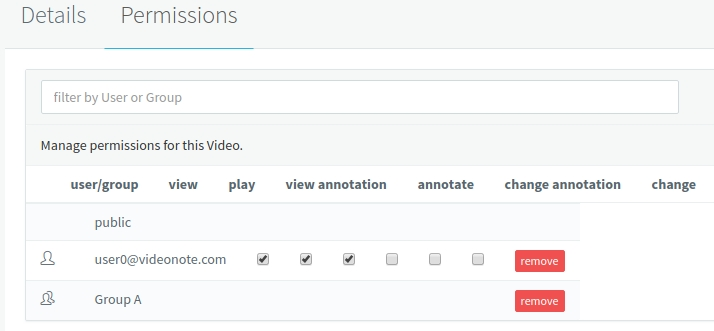
\includegraphics[width=0.9\textwidth]{images/permissions.jpg}
  \caption{Разграничение доступов к видеофайлу}\label{permissions}
\end{figure}

\FloatBarrier

\subsubsection{Проверка ограничения доступа}

Динамически определенные атрибуты позволяют вызвать у менеджера доступа AccessManager методы check\_something и apply\_something,
где something — любое допустимое имя. Это имя служит именем способности — ability — которая запрашивается у системы.
Например, для получения прав на просмотр (способность visible), запрашиваются методы check\_visible и appy\_visible.

Метод check\_something получает модель и определяет ограничение способности в ее отношении, а методу appy\_something
передается QuerySet и метод определяет ограничения нашей способности относительно списка объектов в этом запросе.

Менеджер ищет зарегистрированный плагин и запрашивает у него, либо у плагина по умолчанию, аналогичный метод.
Отсутствующий метод означает разрешение запрошенных действий с указанной способностью в отношение всех объектов
запрошенного множества. Если плагин найден, он и осуществляет проверку.

\subsection{Элементы пользовательского интерфейса}

В ходе анализа существующих решений, а также изучения бизнес требований предъявляемых к системе,
был разработан базовый набор модулей, необходимых для управления платформой видеолекций.

На рисунке \ref{user-interface} представлен фрагмент пользовательского интерфейса приложения.
Видео разбиты по тематическим каналам. Есть возможно оформить подписку на канал - видео с этих
каналов будут отображаться в разделе "My Subscriptions".

\begin{figure}[H]
  \centering
  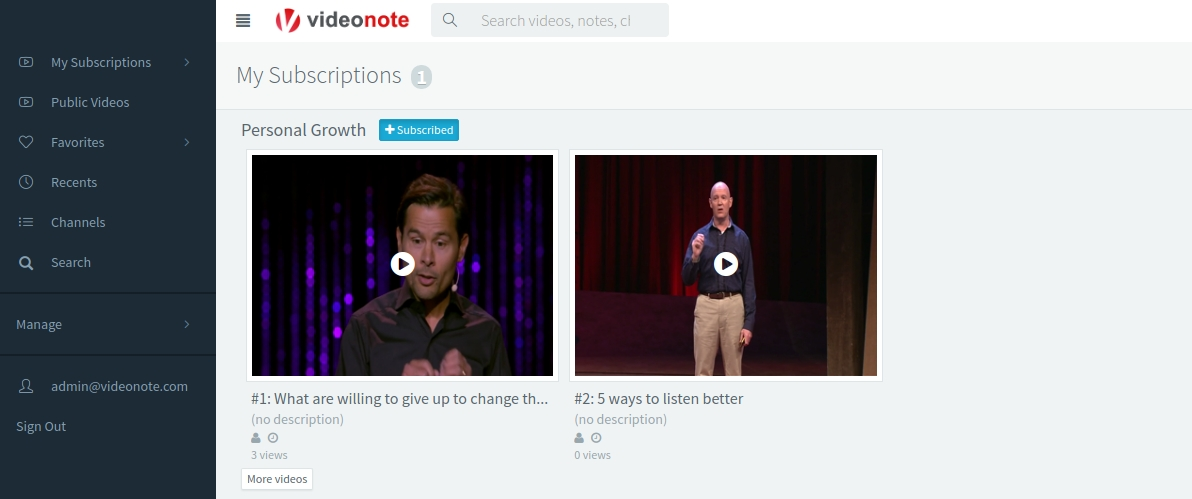
\includegraphics[width=1\textwidth]{images/user-interface.jpg}
  \caption{Список лекций\label{user-interface}}
\end{figure}

На рисунке \ref{annotations} показана страница просмотра лекции. В блоке с аннотациями
выводятся заметки, сгруппированные в секции, привязанные к текущему таймфрему видео.
При клике на секцию происходит переход к соответсвующему фрагменту видео. Здесь же, при просмотре
видео, есть возможность добавления/редактирования аннотаций лектором.

\begin{figure}[H]
  \centering
  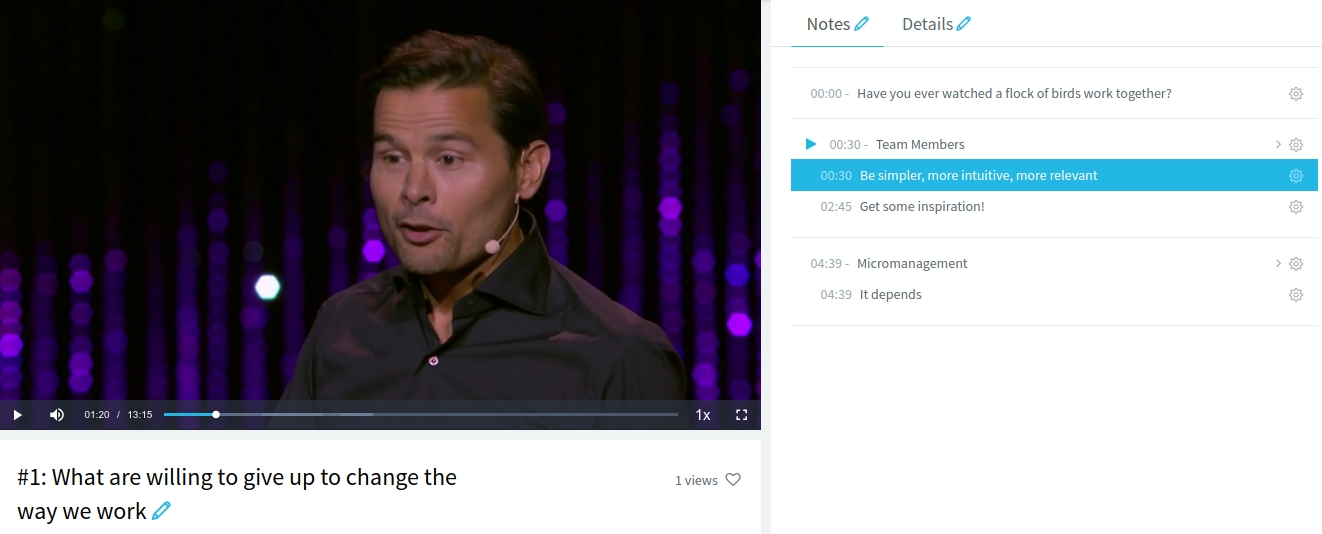
\includegraphics[width=1\textwidth]{images/annotations.jpg}
  \caption{Аннотации при просмотре видео}\label{annotations}
\end{figure}

%\FloatBarrier

\subsection{Полнотекстовый поиск}

Полнотекстовый поиск (Full-Text Search, FTS) это когда вы ищите какие-то документы,
скажем, товары в интернет-магазине или статьи в блоге, по текстовому запросу. в PostgreSQL из коробки есть
полнотекстовый поиск, притом, в отличие от некоторых других РСУБД, очень даже неплохой.

Использовать встроенный в PostgreSQL полнотекстовый поиск вместо связки из PostgreSQL и специализированного ПО для FTS,
такого, как Sphinx, ElasticSearch или Solr, интересно по следующим причинам.
Во-первых, данные не приходится хранить в двух экземплярах. То есть, если у вас 500 Гб данных, не приходится использовать
1 Тб места на диске, что есть удобно. Во-вторых, данные всегда консистентны.
Скажем, если у вас связка из PostgreSQL и ElasticSearch, и синхронизация документов работает с запаздыванием
или ломается, в поиске вы можете увидеть ерунду. Например, уже удаленные документы.
Наконец, в-третьих, не приходится устанавливать и поддерживать какого-либо дополнительного ПО —
обновлять его, бэкапить, мониторить, писать какие-то скрипты синхронизации, и так далее.
Если у вас уже есть PostgreSQL, все просто работает.

Из преимуществ Sphinx, Solr и так далее, следует отметить как минимум то, что будучи специализированными
средствами для полнотекстового поиска, они могут работать быстрее. Хотя бы по той причине, что им не приходится
беспокоиться о транзакциях, проверках целостности данных, и так далее. Если на каком-то этапе развития проекта
вы видите, что скорость полнотекстового поиска в PostgreSQL вас не устраивает, и вы не видите простого способа
это исправить (вертикальное масштабирование, добавить реплик, тюнинг параметров), имеет смысл обратить внимание
на альтернативы. В приложении поиск был реализован с помощью PostgreSQL.

На рисунке \ref{search} отображен блок поиска. Поиск осуществляется не только по названиям лекций,
но и по аннотоациям к видео: секциям и заметкам, а также по каналам. При клике приосходит переход
сразу к каналу, к видео либо к нужному фрагменту видео.

\begin{figure}[H]
  \centering
  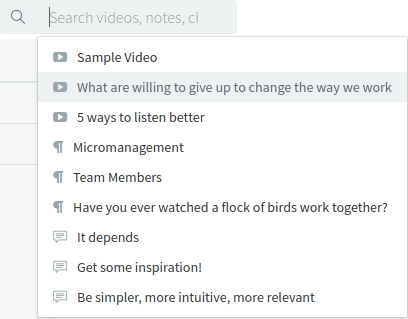
\includegraphics[width=0.7\textwidth]{images/search.jpg}
  \caption{Поиск}\label{search}
\end{figure}

Для интеграции полнотекстового поиска в приложении использовался модуль djorm-ext-pgfulltext. В листинге ~\ref{lst:annotation}
приведены изменения модели аннотации для поддержки полнотекстового поиска. По сути все изменение заключается в том,
что мы добавили search\_index — которое является тем самым tsvector для записи в БД и добавили
новый менеджер запросов в конструктор которого передали следующие параметры:

\begin{itemize}[wide,topsep=0pt]
  \itemsep0em
  \item fields — массив полей из которых будет строиться tsvector;
  \item config — указывает postgresql с каким словарем мы хотим работать;
  \item search\_field — поле в котором у нас лежат данные которые являются уже подготовленным tsveсtor, собранный из указанных в fields полей;
  \item auto\_update\_search\_field — флаг который заставляет пересоздаваться\\ search\_field при изменении записи.
\end{itemize}

Если взглянуть на структуру таблицы, то быдо добавлено одно дополнительное поле — search\_index,
в котором уже лежит tsvector. Это сделано для оптимизации, Postgres умеет работать с уже подготовленными векторами
и не тратить в пустую ресурсы на выполнение to\_tsvector(‘russian’, title||desctription) для каждой строки БД.

\FloatBarrier
\begin{lstlisting}[caption={Изменения в модели аннотации для возможности поиска}, label=lst:annotation]
class Annotation(CreatedByModel):
  time = models.FloatField()

  # enable FTS
  search_index = VectorField()

  search_manager = SearchManager(
    fields=('title', 'description'),
    config='pg_catalog.russian',
    search_field='search_index',
    auto_update_search_field=True
  )

  class Meta:
    abstract = True
\end{lstlisting}
\FloatBarrier

Для выполнения полнотекстового запроса в коде нужно выполнить следующую команду:
\begin{verbatim}
  annotations = Annotation.search_manager.search(query)
\end{verbatim}

где query — это просто строка текста которую мы хотим найти. Естественно к результатам работы этого менеджера
можно применять filter и все остальное.

Стоит добавить пару слов о качестве встроенного полнотекстового поиска PostgreSQL.
Если речь идет о каком то примитивном каталоге товаров — то качество вполне сносное, вполне можно использовать в продакшене.
Если же говорить о более серьезных вещах — таких как поиск текста по предложению — то лучше идти в сторону Elasticsearch, Solr
или Сфинкса.

\subsection{Обработка и доставка видео}

С введением поддержки стандарта HTML5 во многих браузерах стало возможно встраивать видео-плеер при помощи тега video.
Каждый браузер поддерживает определенный набор кодеков и контейнеров. Одним из основных требований к системе являлась
поддержка устройств Apple (iPhone, iPad, iPod). Из-за того, что эти устройства поддерживают онлайн-видео
в единственном формате — MP4 и не имеют возможности использовать Flash-плеер, изначально было решено взять за
основу универсальный MP4-контейнер (H.264 видео и AAC аудио). При кодировании используются бесплатные реализации этих
кодеков libx264 и libfaac. Отсутствие поддержки этих форматов в других браузерах было решено компенсировать
использованием Flash-плеера, который подключается автоматически в случае, если браузер пользователя не поддерживает
тег video, либо поддержка невозможна из-за того, что браузер не поддерживает видео в формате MP4.

Как было описано ранее, доставка контента была реализована с помощью CDN.
Идея в том, чтобы как можно скорее после конвертации переместить файл с основного сервера на файловый,
чтобы избежать скачка нагрузки на сетевом интерфейсе в случае загрузки популярного видео.
Для того, чтобы определить на каком сервере в данный момент находится конкретный видеоролик,
в БД имеется связывающая таблица videofiles.

Архитектура системы по обработки видеофайлов включает 2 типа серверов:

\begin{itemize}[wide,topsep=0pt]
  \itemsep0em
  \item сервер конвертации видео, сбора метаданных;
  \item сервер генерации скриншотов из видео;
\end{itemize}

Для конвертации видео в формат MP4 использовано наиболее популярное в данный момент решение — ffmpeg (\url{http://www.ffmpeg.org/}).
ffmpeg прекрасно справляется с конвертацией видео в самых разнообразных форматах и может использовать несколько ядер
процессора в многоядерной системе. Для пост-обработки была использована утилита MP4Box из пакета gpac (\url{http://gpac.sourceforge.net/}).
Пост-обработка необходима из-за того, что ffmpeg помещает “moov-атомы” (мета-информацию о видео) в конец файла, однако,
чтобы пользователь имел возможность просматривать видео не дожидаясь его полной загрузки, эти атомы должны быть
вначале файла. MP4Box перемещает их в начало и, кроме этого, приводит файл в соответствие со всеми стандартами,
делает его пригодным для потоковой трансляции через соответствующий модуль.

Для каждого видео делаются экранные снимки в определенных моментах времени, чтобы пользователь смог беглым взглядом
оценить содержание ролика, как показано на рисунке \ref{thumbnails}. Из всех сгенерированных снимков
случайным образом выбирается аватар, который служит “обложкой” и отображается при просмотре списка видео. Пример списка
лекций на канале показан на рисунке \ref{user-interface}.

\begin{figure}
  \centering
  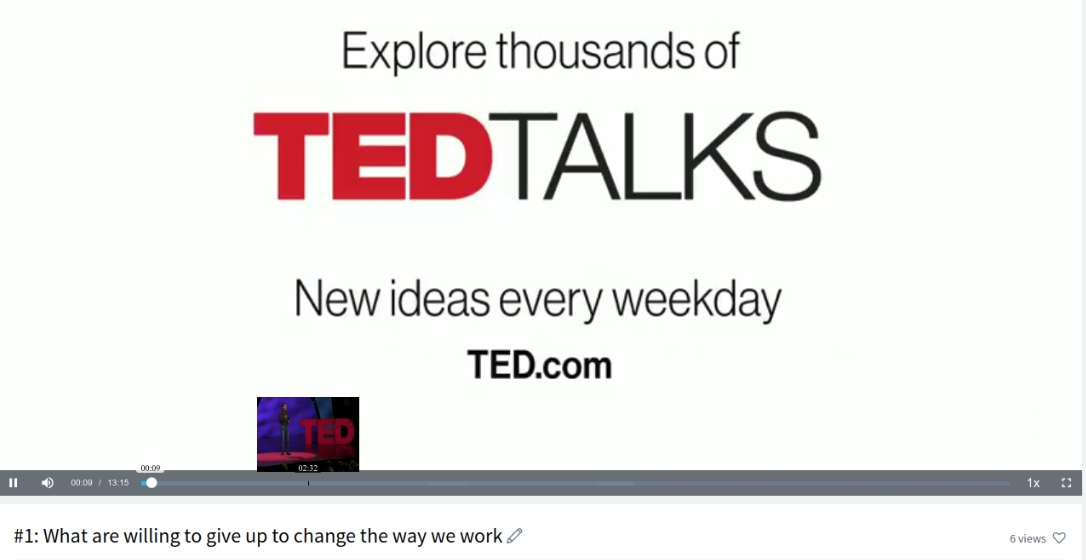
\includegraphics[width=0.7\textwidth]{images/thumbnails.jpg}
  \caption{Оценка содержания ролика по скриншотам}\label{thumbnails}
\end{figure}

\FloatBarrier

Пример использования ffmpeg для генерации экранных снимков:
\begin{verbatim}
cmd = \
  'ffmpeg -i {i} -f image2 -s {w}x{h} -vf
    fps=fps=1/{t} {d}/\%04d.{x}' \
  .format(
    i=input_filepath,
    w=width,
    h=height,
    t=thumbnail_interval,
    d=tn_dir,
    x=ext.lstrip('.')
  )
\end{verbatim}

Обратим внимание на опцию thumbnail\_interval. Она определяет через сколько кадров будет сохранён каждый новый
ключевой кадр (keyframe). Наличие ключевых кадров необходимо также для того, чтобы пользователь мог прокручивать
длинный ролик не дожидаясь его полной загрузки. Эта возможность реализуется при помощи модуля трансляции.
Клиент (браузер или Flash-плеер) передаёт веб-серверу GET-параметр start, который обрабатывается модулем трансляции
и означает количество секунд с которого нужно начинать проигрывание. Кроме того, параметр -threads 0 существенно
увеличит скорость конвертации указав программе на необходимость автоматически определить количество ядер
процессора и использовать их в процессе работы.

На клиентской части был использован VideoJS (\url{http://videojs.com}) для проигрывания и стилизации HTML5-видео.
Кроме того, VideoJS выполняет “более умный” откат к Flash-плееру (в случае отсутствия поддерживаемого браузером видеофайла
в списке источников). В качестве Flash-плеера использован flowplayer (\url{http://flowplayer.org}).

Следует отметить, что всё программное обеспечение собиралось вручную из исходных кодов (клонировалось из соответствующих
систем контроля версий либо использовались свежие сборки). Использование самых новых версии из стабильных веток очень важно
так как с момента исправления какого-либо бага до попадания этих исправлений в пакет выбранного вами дистрибутива Linux
проходит достаточно много времени.
